% HEADER
\documentclass[class=article, crop=false]{standalone}
\usepackage{00_Preamble/frr_preamble}

% Packages
\usepackage{titlesec}
\usepackage{hyperref}
\usepackage{float}
\usepackage{graphics}
\usepackage{placeins}
\usepackage{adjustbox}
\usepackage{array}


\renewcommand{\arraystretch}{1.4}
% END HEADER

\begin{document}
	\subsection{Preliminary Design}
	\label{subsec:preliminary_design}
	Each system on the robot went through multiple design iterations during the preliminary design process. Significant background research was conducted into the Mars environment, potential excavation systems, drivetrain, and path planning and SLAM implementations. Trade studies were combined with testing to determine the best and most realistic rover design.
	\subsubsection{Drive System}
In order to determine the behavior of drive systems in the competition conditions, research was conducted on drive systems used by various teams from previous years. Many robots encountered wheel slippage and struggled to maneuver out of steep ditches. In order to achieve the goal of autonomy, the team aimed to design the drive system to minimize slippage and maximize maneuverability.

Two potential drive mechanisms were considered: a 4-wheel direct drive and tank tread drive. A trade study for the drive systems considered is shown in Table \ref{table:drive_trade_study}. The tank tread drive is superior to the wheeled drive system in traction and obstacle traversal. However, due to the increased number of parts, it is also less power efficient, heavier, and more difficult to manufacture. The 4-wheel direct drive has very few moving components, making system integration and assembly much simpler. However, few off-the-shelf wheels exist that satisfy the design parameters, necessitating the wheels to be custom-manufactured. While a wheeled drive does not have as much traction as the tank tread drive, independent control for all four wheels allows for advanced control algorithms to monitor and correct wheel slippage. Additionally, the system would be fail-operational in the case a of single drive motor failure. Due to the simpler design implementation and independent control of each wheel, the four wheel direct drive system was selected.



\FloatBarrier
	\begin{table}[h]
	\footnotesize
	\centering
	\begin{tabular}{ | p{8em} | m{4em} | m{6em} | m{3em} | m{8em} | m{3em} | }
 	\hline
 		\rowcolor[gray]{0.8}
 		\textbf{Factor} &\textbf{Weight} &\textbf{Tank Tread Drive} &\textbf{Score} &\textbf{4-Wheel Direct Drive} &\textbf{Score}  \\ 
 		\hline
		Fabrication                       &  \multicolumn{1}{c|}{0.7}  &  \multicolumn{1}{c|}{8}    &  \multicolumn{1}{c|}{5.6}  &  \multicolumn{1}{c|}{4}    &  \multicolumn{1}{c|}{2.8}   \\ 
 		\hline
 		Obstacle \mbox{Avoidance}         &  \multicolumn{1}{c|}{0.9}  &  \multicolumn{1}{c|}{7}    &  \multicolumn{1}{c|}{6.3}  &  \multicolumn{1}{c|}{9}    &  \multicolumn{1}{c|}{8.1}   \\ 
 		\hline
 		\mbox{Control System} Complexity  &  \multicolumn{1}{c|}{0.6}  &  \multicolumn{1}{c|}{9}    &  \multicolumn{1}{c|}{5.4}  &  \multicolumn{1}{c|}{6}    &  \multicolumn{1}{c|}{3.6}   \\
 		\hline
 		Power \mbox{Efficiency}           &  \multicolumn{1}{c|}{0.4}  &  \multicolumn{1}{c|}{5}    &  \multicolumn{1}{c|}{2}    &  \multicolumn{1}{c|}{9}    &  \multicolumn{1}{c|}{3.6}   \\ 
 		\hline
 		Obstacle \mbox{Traversal}         &  \multicolumn{1}{c|}{0.7}  &  \multicolumn{1}{c|}{8}    &  \multicolumn{1}{c|}{5.6}  &  \multicolumn{1}{c|}{7}    &  \multicolumn{1}{c|}{4.9}   \\
 		\hline
 		\mbox{Reliability and} Simplicity &  \multicolumn{1}{c|}{0.6}  &  \multicolumn{1}{c|}{4}    &  \multicolumn{1}{c|}{2.4}  &  \multicolumn{1}{c|}{9}    &  \multicolumn{1}{c|}{5.4}   \\
 		\hline
 		\rowcolor[gray]{0.9}
 		\textbf{Total}                    &       &       &\multicolumn{1}{c|}{\textbf{27.3}}&       &\multicolumn{1}{c|}{\textbf{28.4}}\\
 		\hline
	\end{tabular}
	\caption{Trade Study Matrix for Drive System }
		\label{table:drive_trade_study}
	\end{table}
	\FloatBarrier
	
	\subsubsection{Wheels}
	The wheels were designed to find a compromise between traction, obstacle-traversal ability, weight, and build complexity. The preliminary wheel design can be seen in Figure \ref{fig:cad-wheel-prelim}. The wheels have a 30 cm diameter to be able to climb over smaller obstacles. Based on research into rover wheel design, the team determined that grousers were required to provide traction in the loose BP-1. 12 grousers were chosen to be a good compromise between traction and a smooth ride to reduce vibration and sensor noise. The red spacers are 3D printed to fasten the grousers, wheel sides, and rim together. 6061-T6 aluminum was selected due to its low weight, relatively high strength, and machinability.
	
	\FloatBarrier
		\begin{figure}[h]
			\centering
			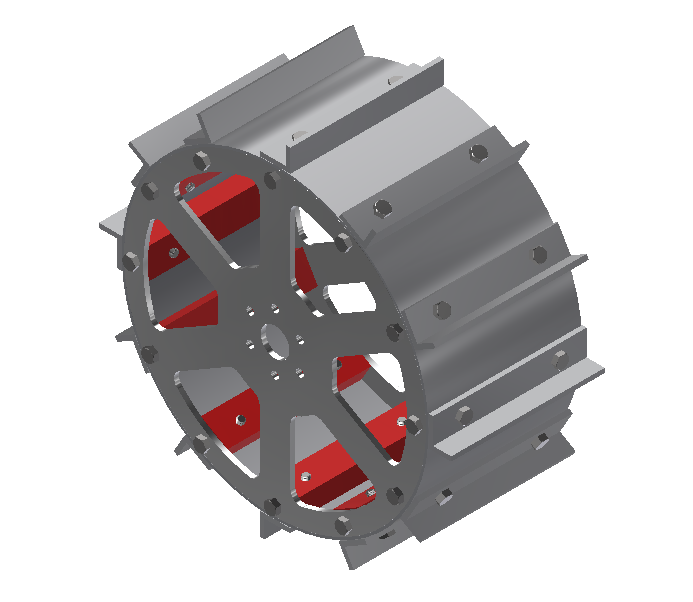
\includegraphics[width=0.4\linewidth]{09_Figures/wheel-cad-preliminary.jpg}
			\caption{CAD model of preliminary wheel design.}
			\label{fig:cad-wheel-prelim}
		\end{figure}
		\FloatBarrier

	\subsubsection{Excavation}
The main requirement for the excavation system was to dig through 30 cm of BP-1 and collect the icy regolith simulant underneath. The primary design considerations for the digging mechanism were reliability, dust tolerance, complexity, and weight. 
Research was performed on existing digging mechanisms in the mining industry. Table \ref{table:dig-trade-study} shows a trade study of potential mining mechanisms. The backhoe and bucket wheel excavator were eliminated from the solution space as they are primarily effective for surface mining. Additionally, the bucket wheel excavator is capable of removing a large amount of material, but does not fit within the size constraints of the robot.
The chain trencher, which consists of a large chain that draws material out of the ground, is capable of achieving a higher rate of gravel removal than an auger. After consulting with engineers at Ditch Witch, it was determined that a chain trencher of the correct scale for the mining robot would require at least 4 horsepower to drive. The increase in mass and energy usage for the chain trencher does not justify the increased rate of gravel collection.

The auger mechanism provides a compromise between weight, power consumption, and the mass of gravel collected. The rate of gravel collection and power consumption can be scaled by the diameter of the auger, allowing the system to be better designed for the robot. Additionally, fabrication and assembly of the auger system is significantly simpler than that for the chain trencher. Therefore, the auger was selected as the excavation mechanism.

Experiments were conducted to test the effectiveness of elevating sand and gravel through a PVC pipe using an auger. The results from the experiment demonstrated that the auger is capable of excavating gravel. Furthermore, it was found that the auger performed best at an angle of approximately 60 degrees. 



\FloatBarrier
	\begin{table}[h]
	\scriptsize
	\centering
	\begin{tabular}{ | r | c | c | c | c | c | c | c | c | c | c |}
 	\hline
 		\rowcolor[gray]{0.8}
 		\textbf{.} &\textbf{Cost} &\textbf{Fabrication} &\textbf{Power} &\makecell{\textbf{Operative} \\ \textbf{Complexity}} &\textbf{Robustness} &\makecell{\textbf{Scoring} \\ \textbf{Potential}} &\textbf{Mass} & \makecell{\textbf{Ease of} \\ \textbf{Integration}} &\textbf{Size} &  \\ 
 		\hline
		\makecell{\textbf{Decision} \\ \textbf{Weight:}}& \textbf{0.1} &\textbf{0.15} &\textbf{0.1} &\textbf{0.05} &\textbf{0.05} &\textbf{0.2} &
		\textbf{0.1} &\textbf{0.1}  &\textbf{0.15} &\makecell{\textbf{\underline{Weighted}} \\ \textbf{\underline{Score}}}  \\ 
 		\hline\hline
 		\makecell{\textbf{Auger and} \\ \textbf{Tube}}    & 8 & 8 & 7 & 8 & 6 & 3 & 6 & 5 & 7 & \textbf{6.15} \\ 
 		\hline
 		\makecell{\textbf{Chain} \\ \textbf{Trencher}}    & 6 & 8 & 1 & 9 & 7 & 10 & 2 & 3 & 2 & \textbf{5.5} \\
 		\hline
 		\makecell{\textbf{Bucket} \\ \textbf{Excavator}}  & 6 & 5 & 4 & 7 & 3 & 1 & 7 & 10 & 6 & \textbf{4.05} \\
 		\hline
 		\makecell{\textbf{Plow and} \\ \textbf{Back-hoe}} & 5 & 5 & 4 & 5 & 2 & 2 & 3 & 2 & 2 & \textbf{3.2} \\
 		\hline
 		\makecell{\textbf{Circular} \\ \textbf{Excavator}}& 5 & 2 & 6 & 8 & 3 & 6 & 2 & 7 & 1 & \textbf{4.2} \\ 
 		\hline
	\end{tabular}
	\caption{Trade Study Matrix for Digging Mechanism}
		\label{table:dig-trade-study}
	\end{table}
	\FloatBarrier
	
	
	\subsubsection{Depositing}
	Once the icy regolith is collected, it must be stored on the robot until it can be deposited in the collection bin. It was determined that it would be easiest to run the depositing system from the end of the excavation system to the back of the robot. The robot can then be driven in reverse to the collection bin and can avoid the wheel slippage that occurs when making large turns. The excavation system will extract a lot of BP-1, which does not count for points in the competition and increases power consumption due to the added weight. It was decided to use a weaved conveyor belt with a mesh aperture that allows BP-1 to fall to the ground while retaining the icy regolith.
	
	
	\subsubsection{Autonomy}
	The autonomy module is responsible for localizing the robot and providing control commands to navigate the robot around the field. Multiple sensor options for localization and obstacle avoidance were researched. 2D/3D LIDAR systems, cameras, Microsoft Kinect (Figure \ref{fig:kinect-pic}), telemetry sensors such as encoders, and inertial measurement units were all considered. These sensors were each evaluated based on performance parameters such as update rate, computational complexity, price, and noise.
	
	LIDAR based systems were considered due to their widespread use in mapping and localization tasks such as self-driving cars. LIDAR produces high-resolution depth maps of the environment and function  well in environments with limited visibility. However, many 3D LIDAR sensors, which produce a three dimensional scan of the environment, are cost-prohibitive and are not feasible within the team’s budget. While some 2D LIDAR systems fall within the budget,they only produce a planar scan of the environment. Since the obstacles on the field are low to the ground, it would be difficult to find a suitable place to mount the LIDAR system on the robot. 
	
	\begin{wrapfigure}{l}{0.5\textwidth}
	\centering
	 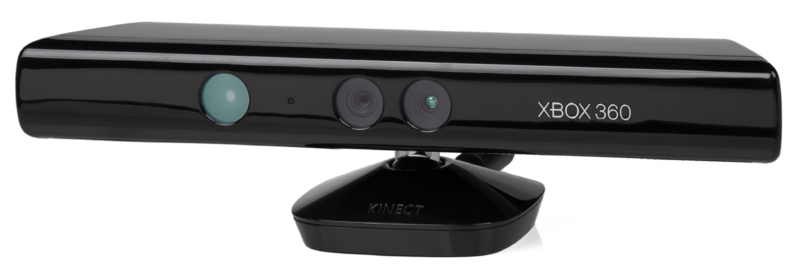
\includegraphics[width=0.48\textwidth]{09_Figures/xbox-360-kinect.png}
	 \caption{The XBox Kinect, V1}
	 \label{fig:kinect-pic}
	\end{wrapfigure}
	
	In order to localize the robot using a camera system, fiducial markers are often placed at a predefined location to serve as a landmark. The robot then determines its pose using a coordinate transformation. The OpenCV library has pre-built functions for determining robot pose by detecting AruCo markers, which are binary square fiducial markers. This method of localization is advantageous because the time required to implement is low compared to other options. However, since the camera is operating in the visual light spectrum, it may be prone to error measurement due to dust kickup. Additionally, ranging with a single camera may not be as accurate because it relies solely on the relative image size instead of time of flight measurements or stereoscopy.
	
	The Microsoft Kinect is a robust, low-cost, 3-dimensional vision system. The Microsoft Kinect outperforms LiDAR systems in dusty conditions due to its use of structured light three dimensional scanning.~\footnote{C. Hall, "Comparing the Performance Of Structured Light Depth Sensors and Traditional Time-of-flight Depth Sensors For Use in a Lunar Mining Environment", Master's, University of Alabama, 2014.} The kinect has an extensive amount of libraries for collecting and utilizing data for depth mapping and feature detection that could be adapted to match the autonomy module requirements. 
	
	An Inertial measurement unit (IMU) measures acceleration and angular velocity at a high refresh rate. However, since double integration is required to estimate position, the error accumulation rate makes the data unreliable. Instead, an IMU can be used in combination with encoder telemetry data on the drive motors to correct wheel slippage error. By comparing the acceleration and angular velocity measurements from the encoder to the expected values based the IMU data, erroneous data can be eliminated and the wheel velocities can be adjusted to correct for slippage
	
	Based on research conducted for each sensor system, it was determined that the best suited option for the robot would be a combination of a Microsoft Kinect, a camera for AruCo marker tracking, an inertial measurement unit, and encoders for telemetry data. The camera, encoders, and IMU will be used to localize the robot while the Kinect will  be used to track obstacles on the field.
	
	\subsubsection{Robot Controller}
	
	The robot controller is responsible for interpreting sensor inputs, controlling motors, and making autonomous decisions. Each of these tasks have  different hardware requirements. Sensor interpretation and motor control require a variety of IO protocols and real-time operation, whereas autonomy requires high computational power and the ability to parallelize operations (see Figure \ref{fig:data-control}). Each of these systems must also maintain low profiles to fit in a restricted space and must minimize power consumption. Multiple low-powered computers were considered:
	\begin{itemize}
	 \item Raspberry Pi provides a high level of community support and computational power, but remains limited by its IO, lack of real-time operation, and ARM architecture.
	 \item Arduinos provide a large amount of IO but provide very little computational power and difficulty interfacing with Linux based controllers.
	 \item BeagleBone Black provides similar IO to an Arduino with Linux support but lacks computational power.
	 \item BeagleBone Blue has the most IO ports and interfaces of the considered controllers. Its layout is designed for robotics applications and for interfacing with common sensors and actuators. 
	 \item The UP Board provides the best computational power whie maintaining the form factor of the Raspberry Pi, but draws substantially more power and retains the Pi’s limited IO.
	\end{itemize}
	
	The BeagleBone Blue was selected to meet the high level of connectivity required on the robot and the UP Board was selected to provide the computational power required by the autonomy module.
	
	The robot controller software must support a high level of performance, interface with open-source robotics software, and run across multiple connected controllers. However, it also must be simple enough to minimize the training time required for novice team members to begin contributing to software development.
	
	Based on these criteria, ROS (Robot Operating System) was identified as the primary software platform for the robot controller. It provides access to an extensive collection of pre-written robot libraries, greatly reducing the amount of code that needs to be written. In addition, ROS provides a network layer for running applications across a network of devices, supporting the requirement of easy communication between devices on the controller’s distributed system. 
	
	ROSMOD, an application developed by the Institute for Software Integrated Systems at Vanderbilt, allows for the development of distributed ROS applications in a graphical user interface. It simplifies code development by abstracting the hardware from the software. All software is ready to run on any device connected to it which meets the software requirements. ROSMOD helps to reduce the large amount of knowledge and boilerplate code required to properly implement distributed systems in ROS. The final decision was made to use ROSMOD to gain the full advantages of the ROS library with an easy way to develop and deploy code.

	\FloatBarrier
	\begin{figure}[h]
	\centering
	 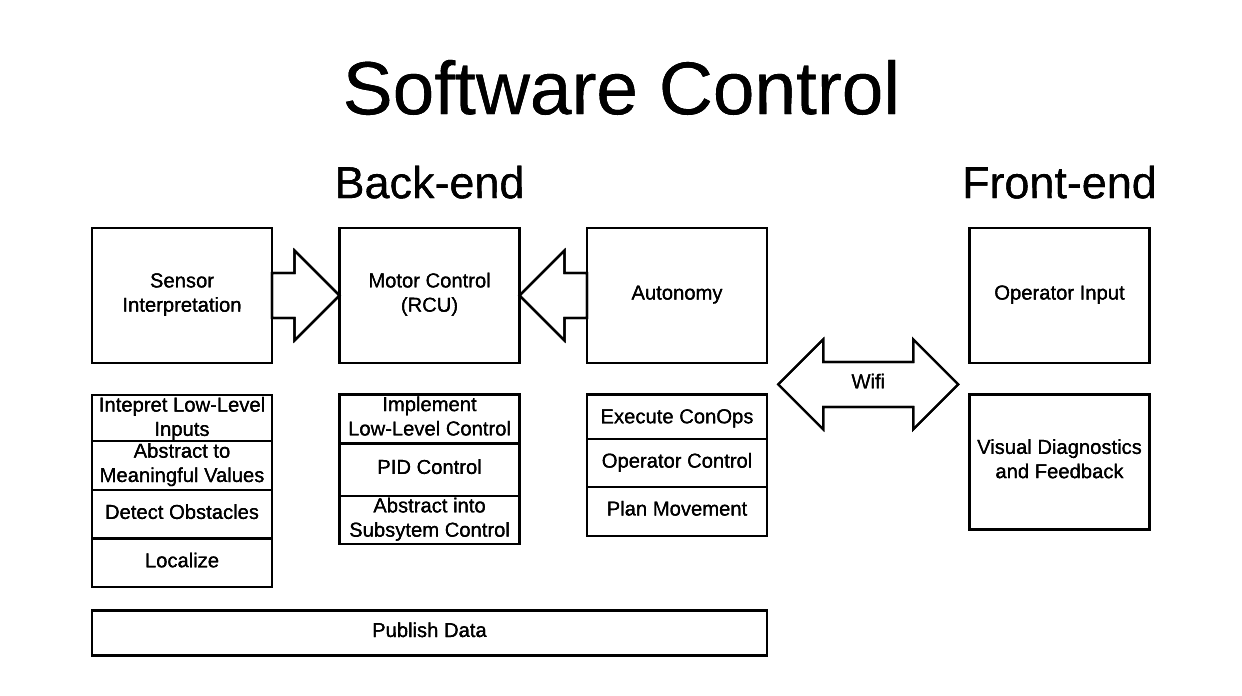
\includegraphics[width=0.8\linewidth]{09_Figures/data-control-high-level.jpg}
	 \caption{Robot Controller flow diagram}
	 \label{fig:data-control}
	\end{figure}
	\FloatBarrier
	
	
	
	\subsection{Preliminary Design Review}
	
	On January 10th, the executive team members met with the team’s faculty advisor to review the proposed preliminary designs. The preliminary design of each subsystem was verified to satisfy the design requirements. The team was cleared to move on the final design stage. 

	
	


	
\end{document}
